\documentclass[a4paper, usenatbib, 12pt]{article}
\usepackage{subfig}
\usepackage{float}
\usepackage{wrapfig}
\usepackage{graphicx}
\usepackage{amsmath}
\usepackage{amssymb}
\usepackage{booktabs}
\usepackage{cite}
\usepackage[icelandic,spanish,english]{babel}
\usepackage[T1]{fontenc}
\usepackage[utf8]{inputenc}
\usepackage[top=3.5cm, bottom=2.5cm, left=3.5cm,right=3.5cm]{geometry} 

%----------------------New commands -------------------

\newcommand{\tol}{Tololo 1214-277}
\newcommand{\lya}{Ly$\alpha$}
\newcommand{\hb}{H$\beta$}
\newcommand{\ha}{H$\alpha$}
\newcommand{\oiii}{[OIII]}
\newcommand{\oii}{[OII]}
\newcommand{\nii}{[NII]}
\newcommand{\esca}{erg cm$^{-2}$ s$^{-1}$ \AA$^{-1}$}
\newcommand{\esc}{erg cm$^{-2}$ s$^{-1}$}
\newcommand{\es}{erg s$^{-1}$}
\newcommand{\esa}{erg s$^{-1}$}
\newcommand{\kms}{km s$^{-1}$}
\newcommand{\apj}{ApJ}  
\newcommand{\jcap}{JCAP}  
\newcommand{\apjs}{ApJS}  
\newcommand{\apjl}{ApJL}  
\newcommand{\aj}{AJ}  
\newcommand{\mnras}{MNRAS}  
\newcommand{\mnrassub}{MNRAS accepted}  
\newcommand{\aap}{A\&A}  
\newcommand{\aaps}{A\&AS}  
\newcommand{\araa}{ARA\&A}  
\newcommand{\nat}{Nature}  
\newcommand{\physrep}{PhR}
\newcommand{\pasp}{PASP}    
\newcommand{\pasj}{PASJ}    
\def\simgt{\lower.5ex\hbox{\gtsima}}
\def\simlt{\lower.5ex\hbox{\ltsima}}
%------------------------------------------------------

\begin{document}
\pagestyle{empty}
\noindent
\textbf{Þú ert jörðin}
\\
\\
JEFR$^{1}$, MCRG$^1$, JNGC$^2$, MG$^3$, MD$^3$
\\
\\
\scriptsize
{$^1$ Bogota
\\
$^2$ Tucson
\\
$^3$ Oslo
\normalsize
\\
\\
\textbf{
  Star-forming Compact Dwarf Galaxies (CDGs) resemble the expected
  pristine conditions of the first galaxies in the Universe.    
Before the observational detection of the first galaxies becomes
reality, CDGs are the best systems to test our ideas on primordial
galaxy formation and evolution.    
Here we report on one of such CDGs, \tol, which presents
a broad symmetric Lyman-$\alpha$ emission that had evaded theoretical
interpretation so far. 
We explain these features by two different models: an
homogeneous sphere undergoing gas bulk rotation and an interstellar
medium composed by clumps with random motions.
It is the first time that an observed \lya\ spectrum can be explained
with these physical conditions.
We  find that both models independently require high velocities that
translate into a dynamical mass at least $10$ times larger than the
neutral mass hydrogen in the galaxy. 
We argue that a possibility to explain the high
dynamical mass is the presence of a super-massive black hole.
The implications of our findings for the study of LAEs, including the
first generation of galaxies are manifold. 
It demonstrates the importance of considering rotation and multiphase
physics under the possible conditions shaping the \lya\ spectra of the
first galaxies. 
Additionally, if future kinematic maps of \tol\ confirm the high
velocities postulated in our model, it would provide new
evidence for dwarf galaxies as hosts of supermassive black holes. 
}  



The first generation of galaxies trace our cosmic origins. 
They were the first steps in the evolution of galaxies such as the Milky
Way. 
In the standard Big Bang cosmology the only chemical elements that
were created in the nucleosynthesis process were Hydrogen, Helium and
Lithium.  
Heavier elements must have been created in stellar evolution process. 
Therefore, we expect the first generation of
galaxies to be metal free and rich in Hydrogen. 
This kind of primordial galaxies have not been detected yet. 
However, dwarf star forming galaxies with a low metallicity content
are seen as templates to understand the early galaxy evolution process. 

Almost fifty years ago \cite{PartridgePeebles} it was realized that
young galaxies could be detected through a strong Lyman-$\alpha$ line
emission.  
This theoretical prediction was only confirmed thirty year later on
distant, relatively young, not primordial, galaxies.
Currently Lyman Alpha Emitting (LAE) galaxies are commonly targeted
in surveys. 
The presence of the Ly-$\alpha$ emission line provides confirmation of
the distance of a galaxy while provides clues about the stellar
population and inter-stellar medium conditions regulating the
Ly-$\alpha$ emission. 

The Ly-$\alpha$ emission line is not exclusive of distant galaxies. 
Any galaxy with low dust content and ongoing star formation has the
right conditions to show this line.  
There are, for instance,  local Universe surveys that target
Ly-$\alpha$ emission in nearby dwarf star forming galaxies 
\cite{LARS}. 
The study of nearby LAE samples has allowed the study of other
indicators that might be more difficult to obtain for distant galaxies
such as morphology, dust attenuation, neutral hydrogen contents and
ionization state.  

However, the physical interpretation of Ly-$\alpha$ observations is
not straightforward. 
This is due to the resonant nature of the Ly-$\alpha$ line. 
A Ly-$\alpha$ photon follows a diffusion-like process before escaping
the galaxy or being absorbed by dust. 
The resulting line profile becomes sensitive to the dynamical, chemical
and thermal conditions in the interstellar medium. 
There are very few analytically tools available to interpret the
Ly-$\alpha$ line.
They are applicable only in very few cases of highly symmetrical
conditions, which are hardly met in real astrophysical systems.
For these reasons the interpretation of Ly-$\alpha$ observations
require state-of-the-art Monte Carlo radiative transfer simulations.   
Recent advances in these computational models have explored the
effects that bulk rotation and a multiphase state in the interstellar
medium should have on on the Lyman-$\alpha$ line.

The most important consequence of bulk rotation is that, even for a
spherical gas distribution, the line morphology now depends on the
viewing angle respect to the rotation axis.  
For a line of sight perpendicular to the rotation axis the intensity
and the line center and the line width increase with rotational
velocity. 
When the rotational velocity is close to the half-line width of the
static line the line becomes single peaked and symmetric, a unique
feature that other theoretical models find difficult to reproduce
without introducing more complexity into the gas distribution. 

This is the case of a multiphase interstellar medium.
The model is more complex as it must take into account the behavior
of neutral dense hydrogen clumps dispersed in a tenuous intraclump medium.  
Corresponding to the elaborate physical conditions in the model,
there are a wide variety of possible emerging spectra.
This variety includes single, double and triple peaked
spectra with different degrees of symmetry around the line's center.


\tol\ is a compact star forming dwarf galaxy that presents a
strong Ly-$\alpha$ emission \cite{Thuan97} with two puzzling 
features: it is symmetric and single peaked.
Commonly, the Ly-$\alpha$ line has a single or asymmetric double peak. 
These two special features in \tol\ had evaded a physical
interpretation so far, because bulk rotation and a multiphase ISM can
independently explain the \lya\ line in \tol. 

Figure 1. summarizes our findings.
Dots represent the observational data for \tol with the
overplot from our best fit models from the full radiative transfer
simulations for a rotating sphere (continuous line) and a clumpy ISM
(dashed line).

The best parameters in the rotation model are a rotational velocity of 
$v_{max}=300^{+xx}_{-xx}$\kms, an optical depth $\log\tau=7^{+xx}_{-xx}$ and a temperature
of $T=1.5^{+xx}_{-xx}\times 10^{4}$K. 
This translates into a column density of $\log N_{HI} /
\mathrm{atoms\ cm}^{-2} =  20.5^{+xx}_{-xx}$.  
This model is also able to constrain the angle between the rotation
axis and the observational line-of-sight to
$\theta=65^{+xx}_{-xx}$$^{\circ}$.  

In the multiphase model the best constrained parameters are
the clump velocity dispersion  $\sigma_{\rm{cl}}=71^{+17}_{-25}$ \kms,
the clumps outflowing velocity $v_{\infty, \rm{cl}}=79^{+167}_{-60}$
\kms and the fraction of the \lya emission that is  coming
from the cold clumps  
$P_{cl}=0.72^{+0.20}_{-0.32}$. 
The multiphase model assumes that the clouds are distributed over a
sphere of $5$kpc in radius, close to the $\approx 4$kpc physical size
of \tol\ as determined by optical imaging.
The assumed physical size and the velocity dispersion $\sigma_{\rm
  cl}$ correspond to a  dynamical mass of  $3.0^{+1.5}_{-1.8}\times
10^9$ M$_{\odot}$. 

Radio surveys of the 21cm line have put an upper limit to the neutral
hydrogen mass in \tol\ of $M<2.65\times 10^{8}$ M$_{\odot}$ \cite{pustilnikmartin07}. 
In the case of the rotation model, this information help us to constrain the
diameter of the HI region where the \lya\ emission and transfer takes
place. 
We find this size to be in the range $0.11 < D/\mathrm{kpc}<0.34$, one
order of magnitude smaller than \tol's size in the optical.   
That size and the rotational velocity of $300$\kms put a constraint on
the dynamical mass of $4.5^{+2.1}_{-2.4} \times 10^{9}$M$_{\odot}$.

This is evidence for a dynamical mass at least 11 (multiphase case) to
17 (rotation case) times higher than the mass in neutral hydrogen.  
There are three main possibilities to explain the dynamical 
mass: stars, dark matter and a supermassive black hole. 
The stellar mass in old stars has been constrained by non-detections
in the K-band to be $<XXX$M$_{\odot}$.
Considering a standard dark matter halo, it can only contribute to
$xx$ M$_{\odot}$ in the region of interest. 
A super massive black hole remains an open possibility. 
Recent observations of ultra-compact dwarf galaxies
\cite{Seth2014} have confirmed the presence of super-massive black
holes containing $15\%$ of the total object mass, suggesting that
there is a large population of undetected black holes in dwarf
galaxies.  


A future observational test to clarify the physical nature of
\tol\ would require integral field unit measurements spatially
resolving its spatial extent. 
\tol\ spans a region of $4$ arcseconds,
an instrument such as the Multi Unit Spectroscopic Explorer with its
nominal $0.2$ arcseconds spatial sampling over a $1.0$ arcminute field
in wide-field mode could provide a coarse mapping of different
ionization lines to infer a kinematic map.
Another observational test includes the measurement of the escape
fraction of Ly continuum ionizing radiation. 
In the rotational model this fraction should be zero, while
the multiphase model predicts that in this case it should be around
$0.5^{+1.0}_{-0.4}$\%. 

All in all, the mere existence of a strong LAE galaxy with a broad,
symmetric line is interesting.
It raises the question whether some high redshift LAEs have asymmetric
lines because the blue half was truncated by the intergalactic medium.
In this case the \lya\ radiation could emerge as a low surface
brightness glow, which may be connected to \lya\ halos, while also
influencing the way LAEs can be used as a probe of reionization. 

These findings demonstrate the importance of including rotation and multiphase
conditions as features to model the \lya\ line in high redshift
galaxies.
Additionally, if the hypothesis of a supermassive black
hole in \tol\ proves to be consistent with future observational
kinematic maps, it could correspond to a so far undetected black hole
in a dwarf galaxy, providing a new way to test and probe
theories on the co-evolution of galaxies and black holes in the first
generation of galaxies.  

\begin{figure}
\begin{center}
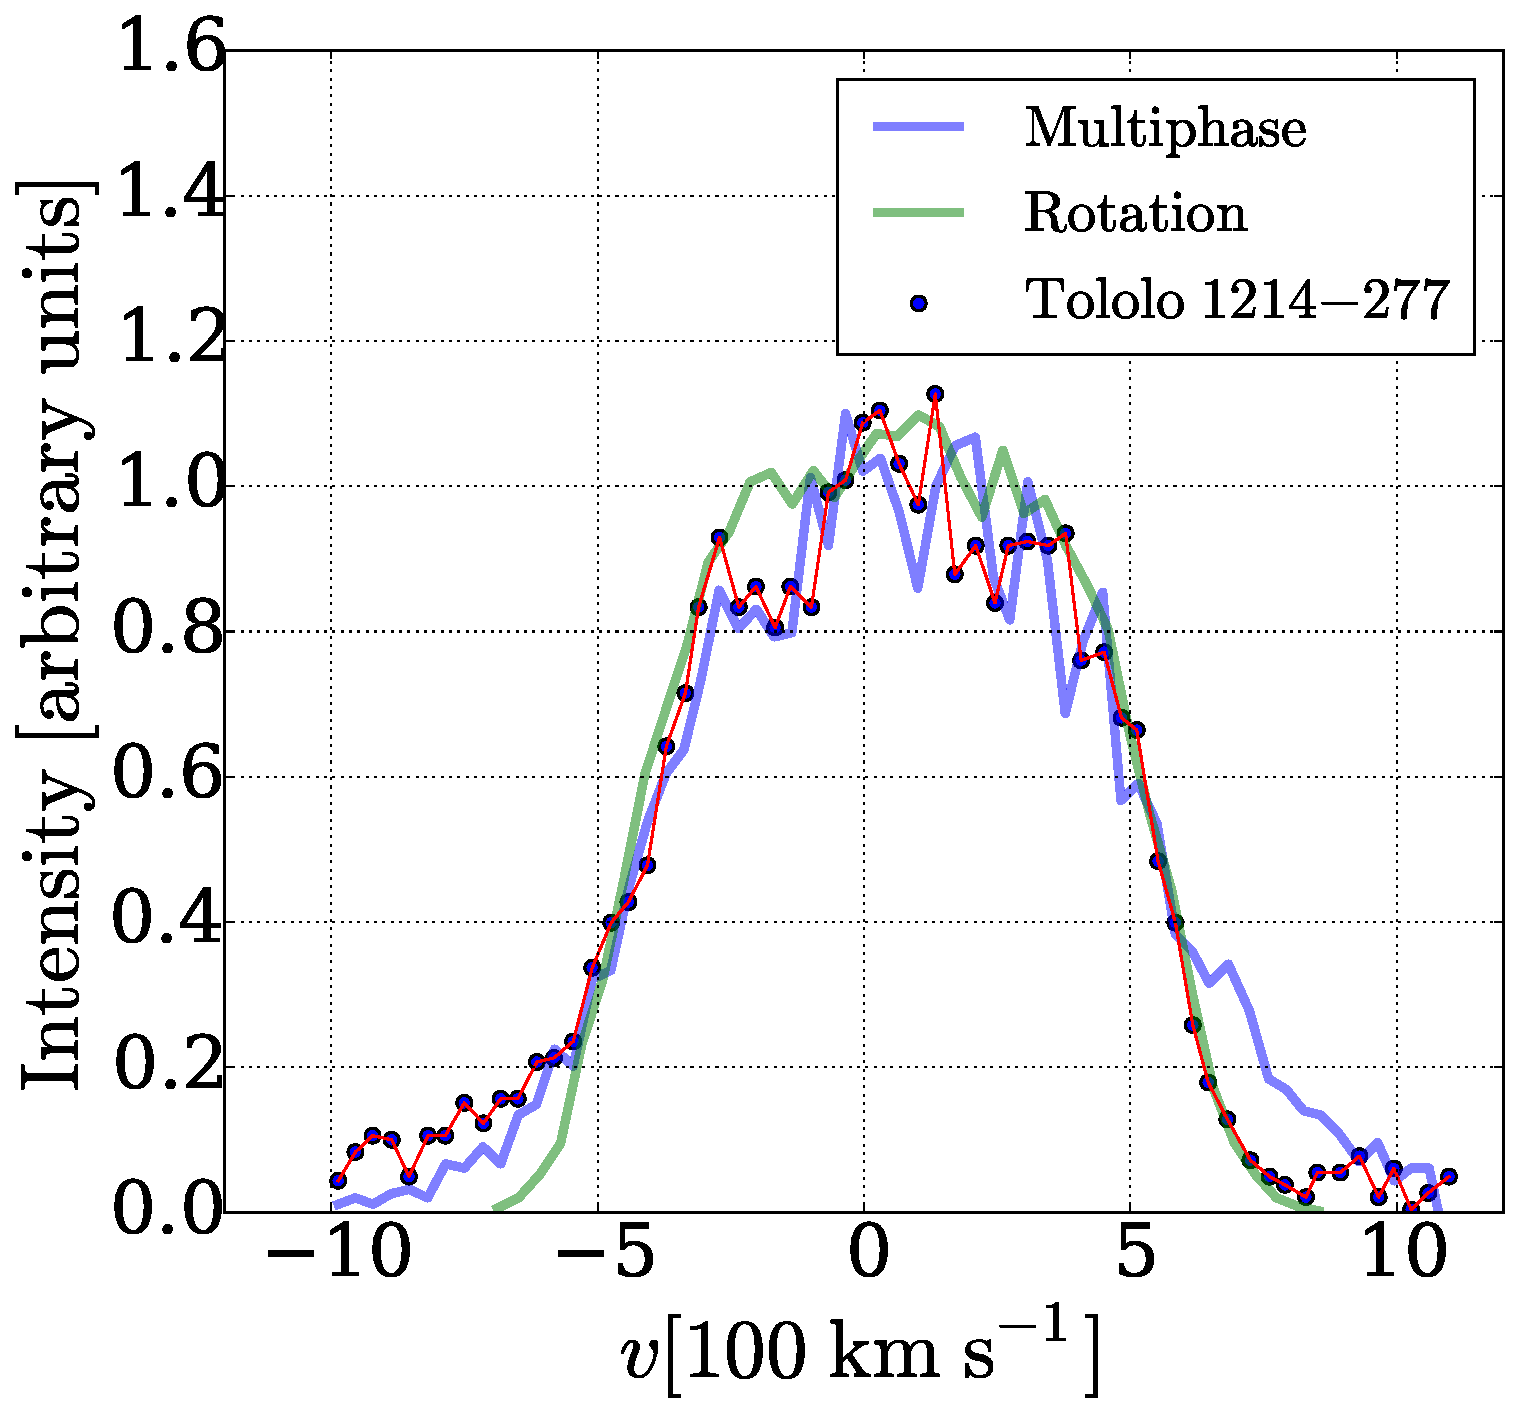
\includegraphics[width=0.8\textwidth]{CLARA-TOL-main.pdf}
\caption{{\bf Broadn, single peaked and symmetric Ly-$\alpha$ emission of \tol.}
  Dots correspond to the observational data. The line shows the results
of our best model from a full radiative transfer simulation both for the rotation and multiphase models.}
\end{center}
\end{figure}

\bibliography{references}{}
\bibliographystyle{plain}

\newpage 

\section*{\tol\ characteristics}


\begin{table}
\begin{center}
\begin{tabular}{lc}
$\alpha$(2000)$^{a}$ & 12h17min17.1s\\
$\delta$(2000)$^{b}$ & -28d02m32s\\
$l$, $b$ (deg) & 294, 34\\
$m_V$ & 17.5\\
  M$_V$ & -17.6\\ 
$v$(km s$^{-1}$) & 7795\\
Ly-$\alpha$ (erg cm$^{-2}$ s$^{-1}$ \AA$^{-1}$)& $8.1\times 10^{-14}$ \\
Ly-$\alpha$ EW & $70$\AA\\
H$\beta$ (erg cm$^{-2}$ s$^{-1}$ \AA$^{-1}$) & $1.62\times 10^{-14}$ \\
$21$cm (Jy km s$^{-1}$)& $<0.10$ \\
\end{tabular}
\end{center}
\caption{Basic observational characteristics of TOL1214-277
  \cite{Thuan97}\\} 
\end{table}

FIXME: Add non detection in 2MASS %\url{http://vizier.u-strasbg.fr/cgi-bin/VizieR?-source=B/2mass}

\tol receding velocity is $7785\pm 50$km s$^{-1}$, which translates
into a distance of $106.6$ Mpc (Hubble constant 73 Mpc km$^{-1}$
s$^{1}$)
Its metallicity is $\sim Z_{\odot}/24$ \cite{Izotov04} as derived from optical
spectroscopy. 


The observed flux for the Lyman alpha line is $\sim
8.1\times 10^{-14}$ erg cm$^{-2}$ s$^{-1}$ \cite{Thuan97}
and a Equivalent Width of $70$\AA and its H$\beta$ flux is 
$1.62\times 10^{-14}$ erg cm$^{-2}$ s$^{-1}$ \AA${-1}$
\cite{Izotov04} which gives a Ly$\alpha$/H$\beta$ flux ratio of
4.9$\pm$0.1. The Ly-$\alpha$ flux values correspond to luminosities of
$L_{Ly\alpha}=2.2\times 10^{42}$ erg s$^{-1}$ over a $20$\AA
bandwidth, which in turns translates  into a star formation rate of
$2.0$ M$_{\odot}$ yr$^{-1}$ using a standard conversion factor between
luminosity and star formation rate of $9.1\times 10^{-43}$
$L_{Ly\alpha}$ M$_{\odot}$ yr$^{-1}$. 
The absolute magnitude in the $V$ band translates into a luminosity of
$8.9\times 10^{8}$ L$_{\odot}$.
% using http://tomdwelly.com/tools_fluxtolum.php
Comparing this ratio with the theoretical expectation from case B
recombination of $23.3$ \cite{Hummer1987} one can estimate an escape
fraction of $20$\% for Ly$\alpha$ radiation.

The optical emission  comes from a   region with approximate diameter
4 kpc \cite{Fricke01}. 

\section*{MCMC constraints}

\section*{Physical Interpretation}

Interpretation by \cite{mashesse03}.

There is an upper limit for the  
integrated flux of $<0.10$ Jy km s$^{-1}$, which translates into a
upper limit for the HI mass of $M<2.65\times 10^{8}$ M$_{\odot}$
\cite{pustilnikmartin07}. 
From the optical depth of $10^7$ and the non-detection in the HI line,
we have an upper limit for the size where the Lya emission comes of
$D<0.34$kpc. 

 For an homogeneous sphere the HI optical depth from its can be
 written as $\tau = \sigma_0 n D/2$, where $\sigma_0=5.898\times
10^{-14}$cm$^{-2}$ is the Lyman$\alpha$  optical depth at the 
line's center, $n$ is the number density and $D$ is the sphere's
diameter. 
From this we can impose additional constrains on $D$ from the typical
values of the Hydrogen number density and our constrain on
$\tau=10^{7}$.  Using a range of $1<n/\mathrm{atoms/cm}^{-3} <
10^{-3}$. This gives us a range of $0.11 < D/\mathrm{kpc}<100$. 
Together from the total HI mass we have thus that the HI region should
have a diameter of $0.11 < D/\mathrm{kpc}<0.34$.



This can be rewritten in terms of the gas' temperature $T$ and column
density $N_{H}$as $\tau = 3.31 \times 10^{-14} (10^{4}\mathrm{K}/T)^{1/2}
(N_{H}/\mathrm{atoms\ cm}^{-2})$.  

This allows us to approximate the total hydrogen mass as
\begin{equation}
M_{H} = m_{H}  N_{H} D^{2} = 226\times \tau  \left(\frac{T}{10^4
  \mathrm{K}}\right)^{1/2}\left(\frac{D}{\mathrm{kpc}}\right)^2M_{\odot}
\end{equation}





On the other hand, we have an estimate for the dynamical mass from the
galaxy size $D$ and its rotational velocity $V$:



\begin{equation}
M_{T} = \frac{V^{2}D}{G} = 2.16\times10^{5}
\left(\frac{V}{\mathrm{km\ s}^{-1}}\right)^2\left(\frac{D}{\mathrm{kpc}}\right) M_{\odot}
\end{equation}


From this limit and the rotational velocity of $300$ km/s and the
limit in the size $D$ we have limits of for the dynamical mass of
$2.1\times 10^{9}$M$_{\odot}$ $<M_D<$  $6.6\times 10^{9}$M$_{\odot}$.
which is at least $7$ to $25$ times larger than the H$I$ mass. The
mass to luminosity ratio is in turn between $2$ to $7$ times
$L_{\odot}/M_{\odot}$ considering the total luminosity in the $V$
band. 



\end{document}

